%
% Optical Stability In Quantum Networks
%

\section{Optical stability in quantum networks} \label{sec:opt_stab} \index{Optical stability}

\dropcap{G}{iven} that communications links in quantum networks are expected to be optical, an issue of central importance is optical stability when signals from remote sources interfere or interact with local quantum states. For example, in an entanglement swapping protocol (Sec.~\ref{sec:swapping}) forming a part of a quantum repeater network (Sec.~\ref{sec:rep_net}), if the entangling operation between the remotely prepared qubits suffers errors, so too will the prepared distributed entangled state.

If we consider the simplest scenario of employing a PBS (Sec.~\ref{sec:bell_proj}) to implement the entangling operation in the polarisation degree of freedom, photon distinguishability in the form of mode-mismatch (Sec.~\ref{sec:MM_error}) will undermine quantum interference, thereby reducing the entangling power of the gate. Similar observations apply to many other protocols involving entangling measurements, or multi-photon interference more generally.

In present-day laboratories, mode-mismatch and photon-distinguishability can be controlled with exceptionally high fidelity. However, in the networking context this is likely to not be so easy, since perfectly aligning states emanating over long-distance communications channels, which we do not have exquisite control over in a well-controlled laboratory setting, is going to be a somewhat unpredictable and time-varying technological challenge.

Such processes are likely to arise in a multitude of ways, including, but certainly not limited to:
\begin{itemize}
	\item Optical fibre: slight variations in temperatures induce refractive index changes, or changes in physical dimension, resulting in temporal displacements of optical wave-packets.
	\item Satellite: precise knowledge of the distance to a rapidly moving target, at the scale of photon wave-packets, is an extremely daunting prospect.
	\item Free space (including via satellite): unpredictable temperature and pressure fluctuations in the atmosphere cause unpredictable variations in the speed of light.
\end{itemize}

For these inevitable reasons, it is important to understand the susceptibility of different network protocols to optical stability. 

There are two dominant forms of photonic interference that must be considered, each with quite distinct behaviours under the influence of optical instability. These are:
\begin{itemize}	
	\item Hong-Ou-Mandel (HOM) interference (Sec.~\ref{sec:HOM_inter}):  interference between two distinct photons at a beamsplitter.
	\item Mach-Zehnder (MZ) interference (Sec.~\ref{sec:MZ_inter}): self-interference of a single-photon traversing multiple paths in superposition within an interferometer.
\end{itemize}

%
% Photon Wave-Packets
%

\subsection{Photon wave-packets} \index{Wave-packets}

Before describing optical interference in detail, we must first formalise a definition for the optical wave-packets we will be dealing with. We will assume wave-packets with Gaussian temporal envelope of width $\sigma$ (the coherence length\index{Coherence length}), frequency-shifted by some carrier frequency $\omega_0$ (the wavelength\index{Wavelength}).

The temporal distribution function is then,
\begin{align} \label{eq:wavepacket_modulated}
\psi(t) = \sqrt[4]{\frac{2}{\sigma\pi}}e^{-\frac{t^2}{\sigma}-i\omega_0t},
\end{align}
with associated mode-operator $\hat{A}^\dag_\psi$ (Sec.~\ref{sec:spatio_temporal}). This wave-packet is normalised such that,
\begin{align}
|\bra{0} \hat{A}_\psi \hat{A}_\psi^\dag \ket{0}|^2 = \int_{-\infty}^\infty |\psi(t)|^2 \, dt = 1.
\end{align}

Of course the temporal envelope needn't be Gaussian in general, and could take any other form, subject to normalisation. In Fig.~\ref{fig:HOM_vs_MZ} we illustrate the two main features of this representation: the temporal envelope, and the underlying carrier frequency that it modulates.

In real-world scenarios we are likely to encounter carrier frequencies sufficiently large that oscillations at the carrier frequency level are far more rapid than that of the temporal envelope. For this simple reason, it is to be expected that interference dependent only on $\sigma$ will be far more robust against temporal instability than interference dependent on $\omega_0$.

\begin{figure}[htpb]
	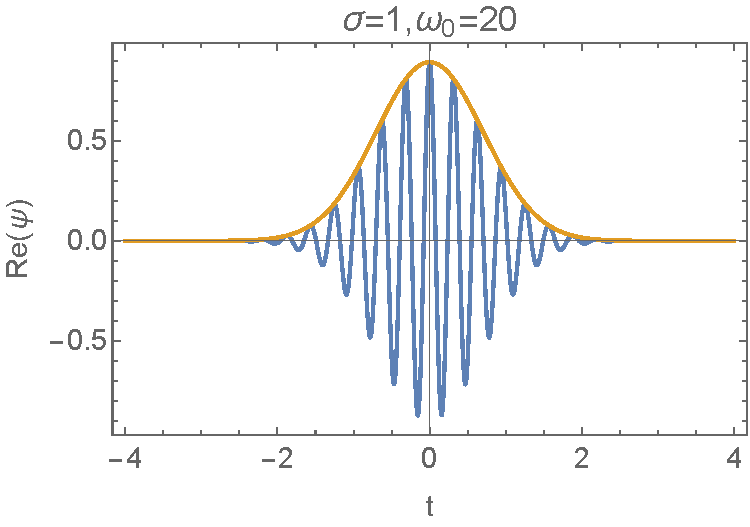
\includegraphics[width=0.47\textwidth]{wavepacket} \\
	\caption{(top) A photonic wave-packet of the form of Eq.~(\ref{eq:wavepacket_modulated}), with Gaussian temporal envelope of width $\sigma$ (orange), shifted by a carrier frequency $\omega_0$ (blue).} \label{fig:HOM_vs_MZ}
\end{figure}

%
% Mach-Zehnder Interference
%

\subsection{Mach-Zehnder interference} \index{Mach-Zehnder (MZ) interference} \label{sec:MZ_inter}

Mach-Zehnder (MZ) interference is the interference of a photon or coherent state with itself in a two-mode interferometer constructed from two 50:50 beamsplitters in series, as shown in Fig.~\ref{fig:MZ_inter}(top). This is MZ interference in its simplest form, which can of course be generalised to more complex networks involving self-interference across multiple optical paths.

Within the interferometer is a time-delay, $\tau$, which acts as a temporal mismatch between the two optical paths. 

\begin{figure}[htpb]
	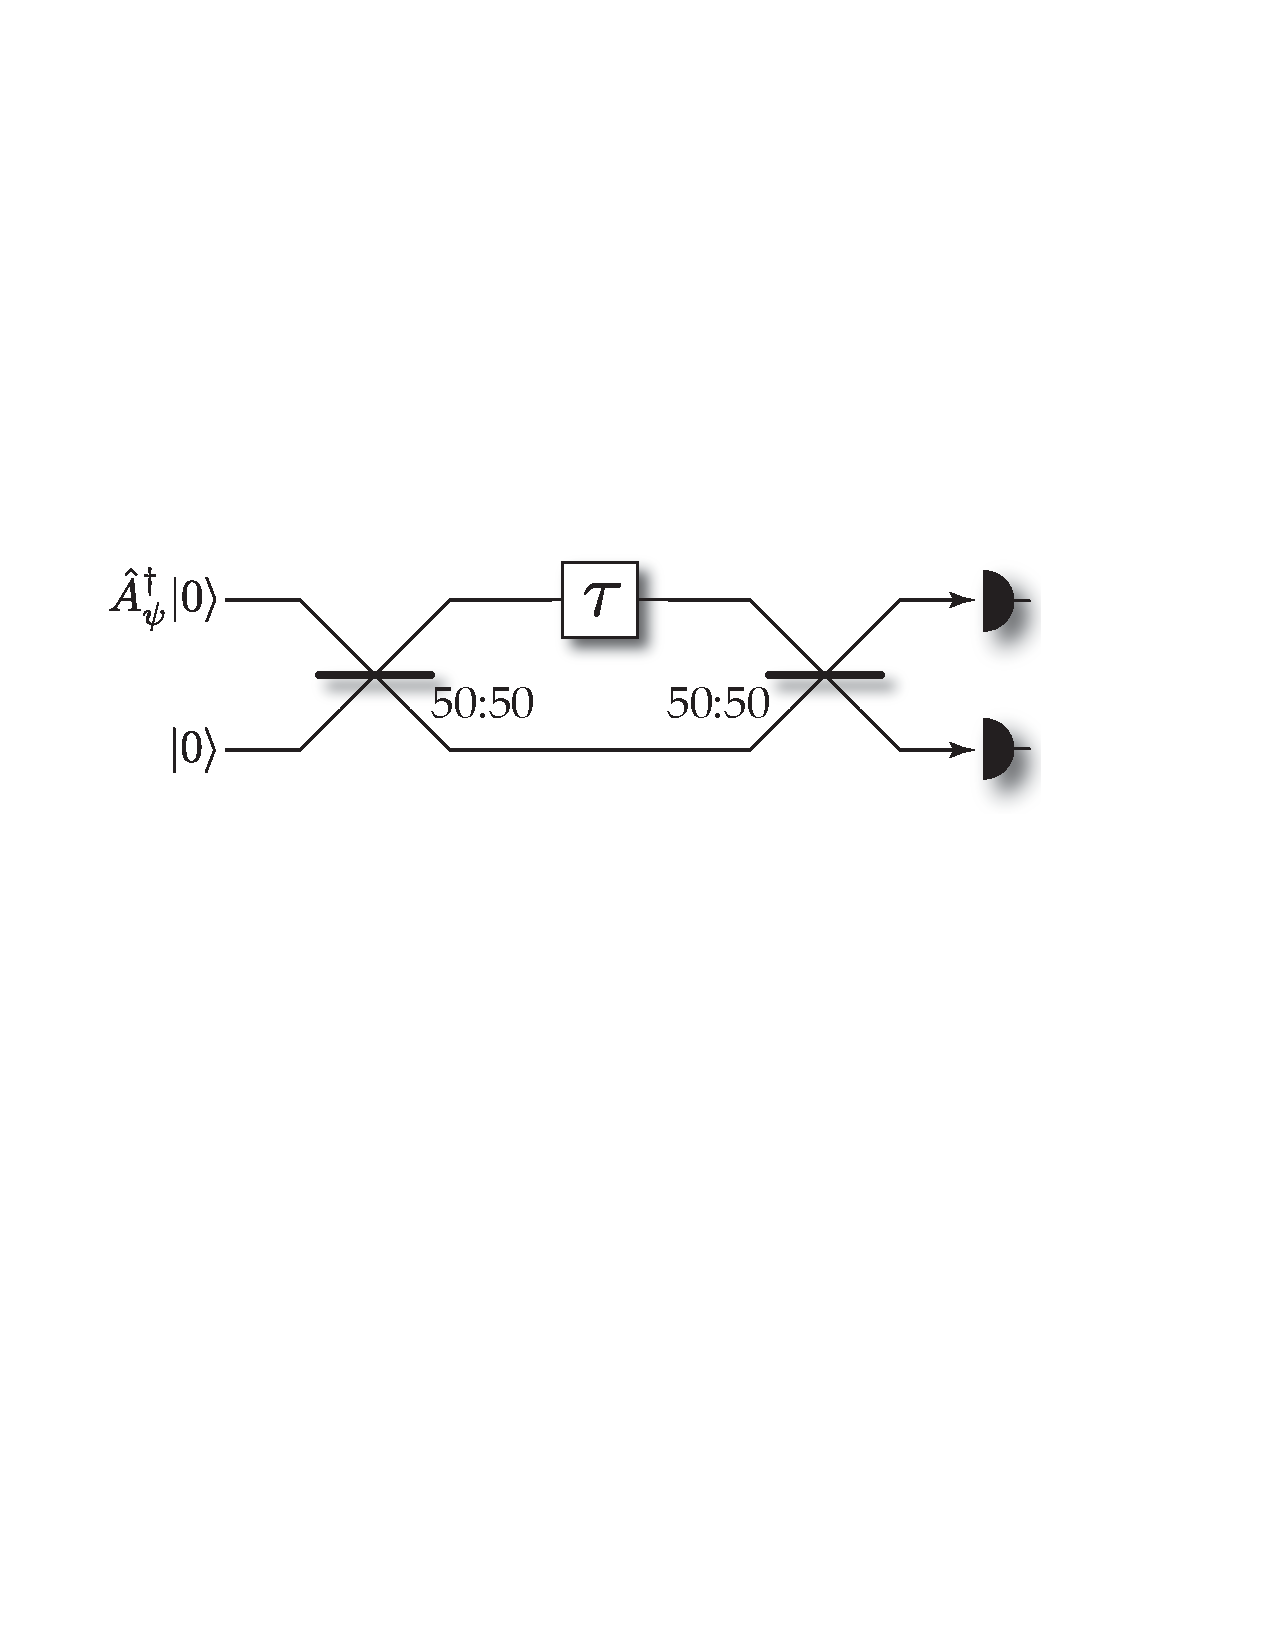
\includegraphics[width=0.47\textwidth]{MZ_setup} \\
	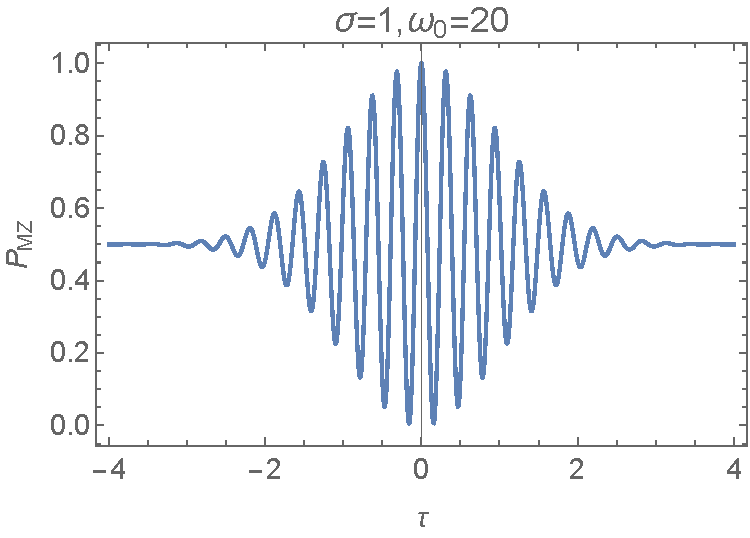
\includegraphics[width=0.47\textwidth]{MZ}
	\caption{Mach-Zehnder self-interference of a single photon. (top) Layout of the interferometer. The photon is subject to a time-delay $\tau$ within only the upper arm of a balanced interferometer, comprising two 50:50 beamsplitters. (bottom) Interference fringe $P_\mathrm{MZ}(\tau)$ as a function of the time-delay. The interference is sensitive at the scale of the photon wavelength, (blue) in Fig.~\ref{fig:HOM_vs_MZ}.} \label{fig:MZ_inter}
\end{figure}

Let us calculate explicitly the evolution of a single-photon through this device, beginning with a photon described by mode operator $\hat{A}^\dag_\psi$\index{Mode operators} (Sec.~\ref{sec:spatio_temporal}), with the temporal distribution function from Eq.~(\ref{eq:wavepacket_modulated}). We have,
\begin{align}
	\ket\psi_\mathrm{in} &= \hat{A}^\dag_\psi \ket{0,0} \nonumber \\
	&\underset{\mathrm{BS}}{\to} \frac{1}{\sqrt{2}} [\hat{A}^\dag_\psi + \hat{B}^\dag_\psi] \ket{0,0} \nonumber \\
	&\underset{\tau}{\to} \frac{1}{\sqrt{2}} [\hat{A}^\dag_{\psi-\tau} + \hat{B}^\dag_\psi] \ket{0,0} \nonumber \\
	&\underset{\mathrm{BS}}{\to} \frac{1}{2} [\hat{A}^\dag_{\psi-\tau} + \hat{B}^\dag_{\psi-\tau} + \hat{A}^\dag_\psi - \hat{B}^\dag_\psi] \ket{0,0} \nonumber \\
	&\underset{\mathrm{PS}}{\to} \frac{1}{2} [\hat{A}^\dag_{\psi-\tau} + \hat{A}^\dag_\psi] \ket{0,0} \nonumber \\
	&= \frac{1}{2} \int_{-\infty}^\infty [\psi(t) + \psi(t-\tau)] \hat{a}^\dag(t)\,dt,
\end{align}
where BS denotes the evolution implemented by a 50:50 beamsplitter, and PS denotes post-selecting upon detecting a single-photon in the first output mode.

We now characterise the operation of the device in terms of the probability of detecting the photon in the first output mode,
\begin{align}
P_\mathrm{MZ}(\tau) &= \frac{1}{4} \int_{-\infty}^\infty |\psi(t) + \psi(t-\tau)|^2 \,dt \nonumber \\
&= \frac{1}{2} \left[ 1 + e^{-\frac{\tau^2}{2\sigma}}\mathrm{cos}(\omega_0\tau) \right].
\end{align}
These dynamics are shown in Fig.~\ref{fig:MZ_inter}(bottom). There are two key features in the behaviour of $P_\mathrm{MZ}(\tau)$. First, there is a slowly varying Gaussian term. Second, the Gaussian term modulates a rapidly oscillating sinusoidial term associated with the carrier frequency. This implies that $\tau$ on the order of the photon's wavelength dominates the measurement dynamics, making it extremely sensitive to temporal instability.

%
% Hong-Ou-Mandel Interference
%

\subsection{Hong-Ou-Mandel interference} \index{Hong-Ou-Mandel (HOM) interference} \label{sec:HOM_inter}

In Hong-Ou-Mandel (HOM) interference, there is no self-interference as per MZ, but rather interference between two independent but indistinguishable photons. The interference takes place at a single 50:50 beamsplitter, with a temporal delay in one input mode modelling temporal instability. The model is shown in Fig.~\ref{fig:HOM_inter}(top).

\begin{figure}[htpb]
	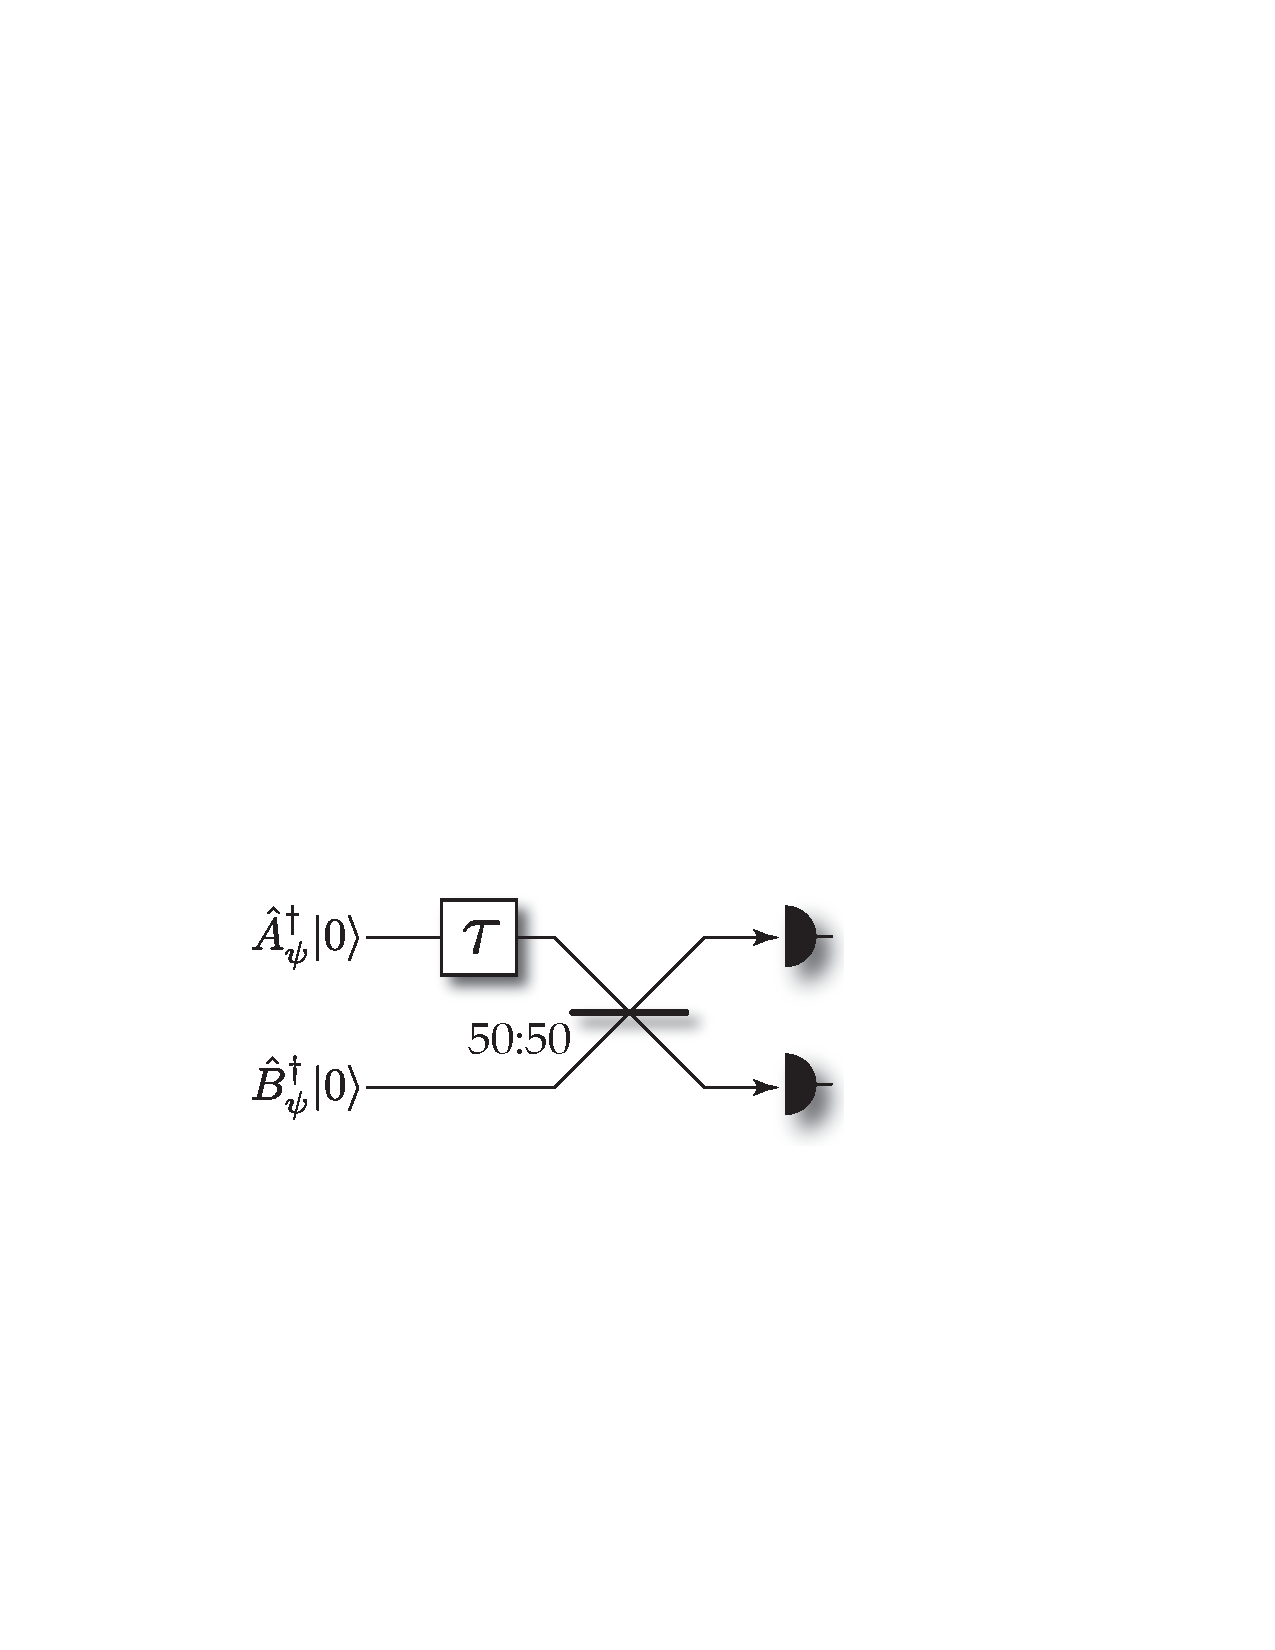
\includegraphics[width=0.325\textwidth]{HOM_setup} \\
	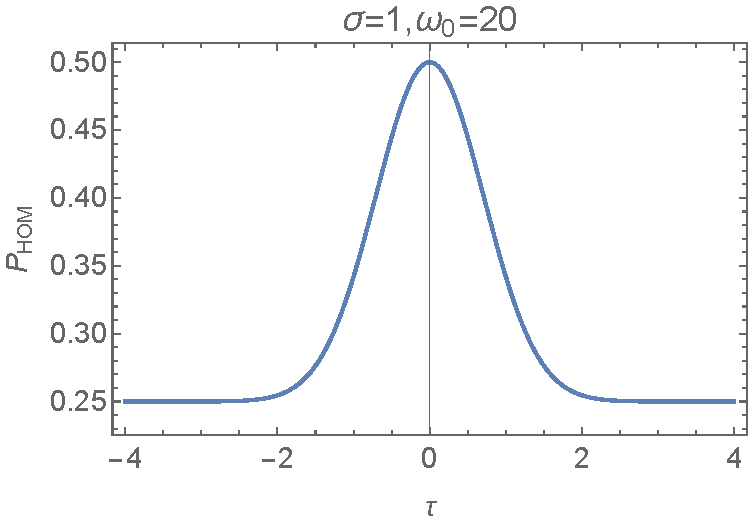
\includegraphics[width=0.47\textwidth]{HOM}
	\caption{Hong-Ou-Mandel interference between two independent photons, $A$ and $B$. (top) Layout of the interferometer. Two photons given by mode operators $\hat{A}^\dag$ and $\hat{B}^\dag$\index{Mode operators} (Sec.~\ref{sec:spatio_temporal}), both with temporal distribution function $\psi(t)$, interfere at a 50:50 beamsplitter, where mode $A$ is first subject to a time-delay $\tau$. (bottom) Interference fringe $P_\mathrm{HOM}(\tau)$ as a function of the time-delay. The fringe is only sensitive at the scale of the wave-packet envelope, (orange) in Fig.~\ref{fig:HOM_vs_MZ}.} \label{fig:HOM_inter}
\end{figure}

Performing the same evaluation of the evolution of the system as before, we obtain,
\begin{align}
	\ket\psi_\mathrm{in} &= \hat{A}^\dag_\psi \hat{B}^\dag_\psi \ket{0,0} \nonumber \\
	&\underset{\tau}{\to} \hat{A}^\dag_{\psi-\tau} \hat{B}^\dag_\psi \ket{0,0} \nonumber \\
	&\underset{\mathrm{BS}}{\to} \frac{1}{2} [\hat{A}^\dag_{\psi-\tau} + \hat{B}^\dag_{\psi-\tau}] [\hat{A}^\dag_\psi - \hat{B}^\dag_\psi] \ket{0,0} \nonumber \\
	&\underset{\mathrm{PS}}{\to} \frac{1}{2} \hat{A}^\dag_\psi \hat{A}^\dag_{\psi-\tau} \ket{0,0} \nonumber \\
	&= \frac{1}{2} \int_{-\infty}^\infty \int_{-\infty}^\infty \psi(t)\psi(t'-\tau)\hat{a}^\dag(t)\hat{a}^\dag(t')\,dt\,dt'.
\end{align}

We then characterise the operation of the device in terms of the probability of detecting both photons in the first output mode (photon bunching),
\begin{align}
	P_\mathrm{HOM}(\tau) &= \frac{1}{4} \left[1 + \left|\int_{-\infty}^\infty \psi(t)\psi(t-\tau)^*\,dt\right|^2 \right] \nonumber \\
	&= \frac{1}{4}\left[ 1 + e^{-\frac{\tau^2}{\sigma}} \right].
\end{align}
These dynamics are shown in Fig.~\ref{fig:HOM_inter}(bottom). Now, unlike MZ interference, we observe no dependence on the carrier frequency and its associated rapidly oscillating terms. Rather, operation depends only on the temporal envelope, which exists over a far larger time-scale.

Importantly, unlike MZ interference, HOM interference is not applicable to coherent states, which do not entangle or enter into superposition at beamsplitters. The photon bunching effect is unique to single-photons.

The intuition behind the HOM-dip phenomenon is as follows. We know that for identical, indistinguishable photons, an input photon-pair evolves as,
\begin{align}
\ket{1,1} \underset{\mathrm{BS}}{\to} \frac{1}{\sqrt{2}}(\ket{2,0}-\ket{0,2}),
\end{align}
yielding perfect photon-bunching. This bunching effect arises from quantum mechanical interference between the photons. Next imagine that the two photons arrived a long time apart from one another, so long that their wave-packets do not overlap at all. In that instance, the photons do not `see' one another and no quantum interference takes place. Instead, rather than a two-photon quantum interference experiment, we effectively have two independent instances of single-photon experiments, given by,
\begin{align}
\ket{1,0} &\underset{\mathrm{BS}}{\to} \frac{1}{\sqrt{2}}(\ket{1,0}+\ket{0,1}), \nonumber \\	
\ket{0,1} &\underset{\mathrm{BS}}{\to} \frac{1}{\sqrt{2}}(\ket{1,0}-\ket{0,1}).
\end{align}
Note that each of these independent instances obeys the classical statistics of a 50/50 distribution. Combining the two instances using classical probability theory, we now observe a 50\% chance of measuring a coincidence, as opposed to the 0\% chance for true HOM interference.

%
% HOM vs MZ Interference
%

\subsection{HOM vs MZ interference} \index{Mach-Zehnder (MZ) interference}\index{Hong-Ou-Mandel (HOM) interference}\index{Hong-Ou-Mandel vs Mach-Zehnder interference}

Let us now examine the implications of these different types of interference. The key observation was that MZ is far more sensitive to temporal mismatch than HOM, the former at the scale of the photons' wavelength, the latter at the scale of their temporal envelope, which is far larger.

This leads to the immediate conclusion that network protocols relying on HOM interference will be far more robust against temporal instability than those relying on MZ interference. Realistically, it is to be expected that the latter might be impossibly challenging in many contexts, as wavelength-scale stabilisation over long distances seems implausible.

In Table.~\ref{table:summary_inter} we summarise the network protocols discussed in Sec.~\ref{sec:protocols_quant_int} in terms of the types of interference they rely upon. This creates a picture of which are more realistic from a near-term engineering perspective.

\begin{table}[htpb]
	\begin{tabular}{|c|c|}
		\hline
  		\rowcolor{Dandelion} Protocol & Interference type \\
  		\hline
  		\hline
  		\rowcolor{LimeGreen} Cluster state measurement & None \\
   		\rowcolor{LimeGreen} Quantum anonymous broadcasting & None \\
  		\rowcolor{LimeGreen} QKD (BB84, E91) & None \\
  		\rowcolor{LimeGreen} Quantum memory & None \\
  		\rowcolor{LimeGreen} Quantum process tomography & None \\
  		\rowcolor{LimeGreen} Quantum state tomography & None \\
  		\rowcolor{LimeGreen} Random number generation & None \\
  		\rowcolor{LimeGreen} Separable measurements & None \\
  		\rowcolor{LimeGreen} Separable state preparation & None \\
  		\rowcolor{LimeGreen} Optical interfacing & None \\
  		\hline
  		\rowcolor{Apricot} Cluster state preparation (fusion gates) & HOM \\
  		\rowcolor{Apricot} Entanglement purification & HOM \\
  		\rowcolor{Apricot} Entanglement swapping & HOM \\ 
  		\rowcolor{Apricot} Matter qubit entangling operations & HOM \\
  		\rowcolor{Apricot} Partial Bell state measurements & HOM \\
   		\rowcolor{Apricot} Quantum gate teleportation & HOM \\
  		\rowcolor{Apricot} Quantum state teleportation & HOM \\
  		\rowcolor{Apricot} Superdense coding & HOM \\
  		\hline
  		\rowcolor{Lavender} \textsc{BosonSampling} & MZ \\
  		\rowcolor{Lavender} General linear optics networks & MZ \\
  		\rowcolor{Lavender} Universal LOQC (KLM) & MZ \\
  		\rowcolor{Lavender} Quantum metrology & MZ \\
  		\rowcolor{Lavender} Quantum walks & MZ \\
    	\hline
	\end{tabular}
	\caption{Summary of the major quantum network protocols presented in Sec.~\ref{sec:protocols_quant_int}, and their required type of interference.}\index{Interferometric requirements}\label{table:summary_inter}
\end{table}

%
% Optical Stabilisation
%

\subsection{Optical stabilisation} \index{Optical stabilisation}

\comment{To do!}

\comment{Discussion of both static and dynamic stabilisation}